\begin{document}
\section{Literature Review}

\subsection{Big Data \& Machine Learning}
Big data is a term used to describe data sets that are considered to be ‘heavier’ than traditional data sets. This can characterised by features such as high frequency of data, large volume or structural diversity [5]. In the context of the smart parking application described in [4], this is due to high frequency of data. Once considered only relevant to certain fields, big data analytics is now recognised to have applications across many areas such as manufacturing, retail, smart cities, and Health etc. This is brought about by the yearly increase of sensors at 30\% in the previously mentioned fields [6].  

 

[7] concurs with the notion that big data possesses characteristics such as frequency, volume and diversity.  They extend this further to describe the process to convert big data into ‘smart data’, which is something that allows effective decision-making. There are several data models such as neural networks, clustering, regression, which can be supervised, unsupervised or semi-supervised. Once the correct model has been identified, algorithms can be applied to the data set to train the Machine Learning Model using the data. This is the general process but there are finer details such as cleaning of data to prepare it for use, evaluation of the model and tuning the model for best fit [8].  Below is a visual overview of the machine learning process for a supervised model. This process has not included the extraction, transformation and loading (ETL) stages and focuses instead on training and inference of machine learning models. 

%
%ADD FIGURE
%
    \begin{figure}[H]
      
      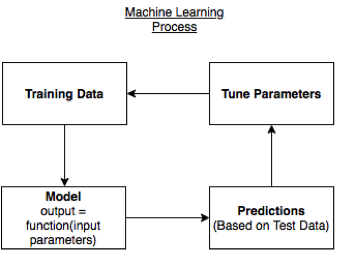
\includegraphics[scale=1.5]{images/MLDiagram.png}
      \caption{Machine Learning Flow}
      \label{fig:Spark}
          
    \end{figure}

The dataset is randomly split into training data and test data (80:20 split respectively is a typical proportion). Machine learning algorithms are used to create a model, which can predict output variable/s as a function of input variable/s. The accuracy of the model is checked using the test data, where the differences are found between the predicted value and the actual value of the output variables. The parameters in the model are then tuned/adjusted to, loosely speaking, be a more accurate fitting model. The key difference between supervised and unsupervised learning is whether there is a predictor/output variable in the model. For example, prediction of the exam marks of a university student by looking at their assignment scores is a supervised model. The input variables are typically referred to as features and the variables to be predicted are labels. 

 Unsupervised models do not have predictor variables but are based upon clustering of data to draw inferences within the dataset. For example, consumers might purchase different things online. The persons who bought item A might also be very likely to buy item B. This kind of analysis is widely used in e-commerce for marketing purposes, with complex algorithms used to make inferences. 

Most of the models found in real life tend to be semi-supervised, employing a mixture of both approaches to train their machine learning model. Machine learning algorithms/data models are chosen based on the type of data that they are applied to, also taking into consideration what kind of output is expected. Time Series modeling is popular in solving transportation problems. It is an appropriate way to analyse and predict parking spaces, which is the desired outcome of this project.   

Another thing to consider is whether the problem is one of Classification or Regression. Classification problems are very popular, especially in the fields of image detection. The key point of difference between a classification  problem and regression problem is the type of prediction made. Classification makes a binary or multivariate prediction while regression predicts a real number value.  For example a classification problem in the space of smart parking would be to identify whether a single car park is likely to be occupied at a given time. This project however looks to solve a regression problem, where the aim is to predict the number of parking spaces occupied at a given time.  

For the use case of smart parking predictions, it is useful to look at the two scenarios mentioned in [9]. In this paper, prediction of parking space availability is noted as being critical to management of traffic within the city. It also results in more efficiency in travel, saving fuel emission if users can find parking spaces in a quick time frame. The first scenario is predicting the interval of time that a particular parking space is free for. The second is generally specified as the total number of parking spaces available in an area, at given time intervals. Both use cases require  predictive regression models; therefore, a Supervised Machine Learning Model is required.  

 

A commonly used prediction model is ARIMA, which is a very easy model to develop and compute. ARIMA is broken down into the processes Auto-Regression (AR), Integration (I) and Moving-Average (MA).  AR is used to fit a regression model for p parameters, while MA is essentially a time window, which models for errors made in d previous predictions. It is the integrator process, which calculates the differences between the prediction and actual value for q time instants, hence also known as difference process.  Hence the relationship is defined below, where y is the prediction value.  
\begin{equation}
    y= ARIMA(p,d,q)
\end{equation}

There are certain limitations to using such a model. This model is only applicable if the time series is stationary and linear. A stationary time series is defined by the overall stability of the distribution. This can be characterised by the parameters such as the mean, median and variance . If the distribution of data is fairly constant, the time series is said to be stable.  In a transportation problem such as parking occupancy this may not hold to be true as there can be a long-term shift in the data caused by several factors such as car ownership rates, location of the car park etc. Linearity in a time series is generally defined to be when each data point is said to be a linear combination of the present value and past values. This results in a correlation between the data points in the time series, thus allowing for AR to take place. The important point to note for car park occupancy modeling is that there can be unexpected changes in the occupancy levels due to large events such as sports games and public holidays. There is also a certain randomness created by events like funerals in the area, which are very difficult to predict. These factors can result in non-linear behavior, which ARIMA cannot account for. Another point to account is that some behaviors previously mentioned are non-deterministic; therefore something must be done to account for those. Any ARIMA model would therefore have to predict values within a range. A more accurate model would result in a smaller range (upper and lower prediction bands would converge). Another point of concern is that the ARIMA model is very sensitive to seasonality, which can be a common behavior in some time series [9-13]. The most popular alternative mentioned by  [9-13] is Artificial Neural Networks (ANN). The networks are referred to as artificial because they are computing models inspired by the way biological neural networks process information [14].  ANN can work with non-linear data that is not stationary and a recurrent layer is useful for quick short-term predictions. There are several variants of ANN, but the one to be considered here is a Deep Neural Network (DNN).  This means that the DNN is a feed-forward (one way traffic) network with a recurring loop (iterations) [10].  DNNs can be categorized as having 3 parts. The first is an input layer, which contains all the parameters. Training Data is fed through the input layer. Each input parameter is a node. The second part is one or more hidden layers. Each hidden layer contains "neurons" which represent computation to take place.  Each node of the input layer is connected to the neurons in the hidden layer and has a certain weight W. The output value of each neuron N is described in the following relationship:



% Black magic way to use images as equation
\begin{center}
          
  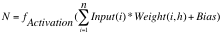
\includegraphics[scale=0.8]{images/equation.png}
              
\end{center}

\begin{flushright}

(2)
\end{flushright}




\subsection{Distributed Computing Framework}
    \begin{figure}[H]
      
      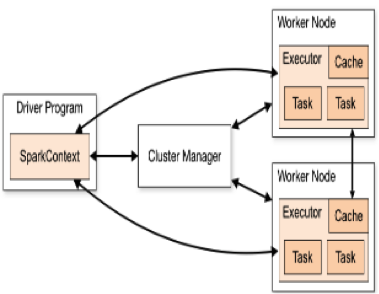
\includegraphics[scale=1.5]{images/Spark.png}
      \caption{Spark Distributed Framework}
      \label{fig:Spark}
          
    \end{figure}


There are several architectures that can be used for distributed computing. An existing architecture solution is a fog based one. According to [2], the fog layer consists of nodes traditionally used as medium throughput nodes. They therefore do not support big data operations (cloud systems are used for big data operations as they require high throughput devices). To support big data through a distributed system, a computational framework is required. Apache Spark is one such framework. Spark uses a driver-worker architecture, which is described in the official documentation as follows [17]. The main program is located in the SparkContext object, which is contained by the driver program. The driver program connects to the cluster manager, which is responsible for managing the combined resources of the cluster. Spark supports many different resource managing applications such as Yarn, Mesos and Spark Standalone. The driver program acquires executors, which are responsible for running the tasks in the application (doing all the computation).  Once the executors have been acquired tasks are sent to them by the SparkContext to run. The cluster manager must therefore address the following issues. Firstly job/task scheduling is required to control the allocations of resources both within applications and across applications. The partitioning of resources can be done using static configuration (Executors are all retained for the life of the program, including their memory) or dynamic configuration.  

Features of Spark: Spark is polyglot, does in-memory computations and contains application programming interfaces (APIs) for machine learning and querying databases amongst others.  

[18] abstracts this driver-worker architecture to a generic master slave architecture. It extends the hierarchy of master (known as driver) by proposing the use of sub-masters, which can be controlled via switches. This is done for scalability. This approach however will require dynamic partitioning of resources.  

[19] uses the Spark Framework to implement a Java Native Interface (JNI), which can also be used to implement hardware accelerators.  

Structured streaming is the way data is sent from the edge nodes to the fog layer [17,19].  It is a processing engine built on Spark SQL. Using Apache Kafka, a broker-subscriber model can be used by the fog layer to ingest data points. Processing ‘batches’ of data is considered to be a more consistent way than using existing frameworks such as Map-Reduce, as events occur in a sequential stream. Another advantage of using structured streaming is that there is always an output (sink) for every input (source), which makes it useful for fault tolerance. It is also useful for data that arrives out of order [20]. The data can also be stored in a distributed file system such as Hadoop Distributed File System (HDFS). 

\subsection{Cloud vs Distributed}

Cost is arguably the most difficult to compare. This is due to the wide range of providers in the cloud computing space and the variance in their offerings. 

[16] details a pricing example. According to the pricing model detailed, the price depends on the following factors: memory, number of virtual machines (VMs), storage and ethernet. The cost is then charged per time unit (typically per hour). Because there is a service level agreement, the promised metrics must be met, guaranteeing quality. Should the vendor fail to abide by the agreement, the tenant can claim free use. 

The pricing model can be either coarse-grained or fine-grained. Cloud computing is famous for a ‘pay as you go’ model. That is the fine-grained pricing mechanism, which charges only on resources used, and charges per smaller time units. The per unit cost of a fine-grained model is higher as a result. The coarse-grained mechanism is comparatively cheaper per time unit but uses large time units and charges for all the resources, whether they are in use for the whole time or not. For example, if only 50\% of memory is used for 15 min out of 1 hour, the full cost is charged for 1 hour. The vendors justify this to cover running costs of operating the VMs. 

 
The majority of large vendors use the Coarse-Grained Model that is very expensive for IoT applications due to the ‘one size fits all’ approach of the model. There are many times where the system does not require as many resources but will have to pay for them anyway. Another reason why cost can be very difficult to determine is that pricing schemes are frequently updated by the vendors and the tenant has to keep an eye on the best deals. Shopping around is difficult due to the technical problems in shifting from one vendor to another. [2] mentions this as one of the many challenges for small and medium enterprises (SME). Maintenance is also an issue for such organizations as there is a requirement for a team of ICT specialists to maintain the operations. This is often not financially feasible for SMEs and so presents a barrier to access the cloud services. 



\end{document}